% TODO: fill in hardware numbers (Table I, and every XX% / XX.X placeholder
% below) once trial collection against the Legged Perceptive Stack completes.

\subsection{Hardware Comparison}
\label{subsec:results-hardware-comparison}

The main evaluation compares GaitNet with the Legged Perceptive Stack
\cite{leggedperceptive} on a physical Unitree Go1. The baseline is a
perceptive NMPC/WBC locomotion framework built on OCS2. It uses fixed
phase trajectories. In the GaitNet condition, we keep the same
NMPC/WBC tracker. We only replace its native gait scheduler with
GaitNet footstep targets
(\autoref{subsec:methodology-system-overview}). The comparison
therefore focuses on the planner, not the low-level tracker.

The test track in \autoref{fig:figure-test-environment} is designed
to match the simulation terrain distribution. Rigid wooden ground
sections are separated by pseudorandom gaps of different widths. We
define terrain difficulty as the percentage of track area that is
unsteppable. It ranges from $\corlDifficultyMin\%$ on flat ground to
$\corlDifficultyMax\%$ on dense gaps. For each method and difficulty
level, we run \corlHwTrialsPerCell{} independent hardware trials. A
trial succeeds only if the robot finishes the track without three
failures: the base touches the ground, the robot drifts off the track,
or a foot lands in a removed terrain section.

We report success rate, traversal time, and total step count. The four
evaluated conditions are:
\begin{enumerate}
  \item \textbf{Legged Perceptive Stack:} the scheduled NMPC/WBC
    baseline \cite{leggedperceptive}.
  \item \textbf{GaitNet-Single:} GaitNet with the contact-count
    constraint tightened so only one leg may swing at a time. This
    matches the concurrency of ContactNet's walking-mode configuration
    \cite{bratta_contactnet_2024}. ContactNet has no public
    implementation, so we use this ablation as a standin for their
    single leg concurrency.
  \item \textbf{GaitNet-Trot:} GaitNet with concurrency restricted to
    diagonally opposing leg pairs, matching a conventional trot
    structure.
  \item \textbf{GaitNet (Full):} the proposed planner. It allows up to
    two concurrent swing legs and does not restrict which legs may
    overlap.
\end{enumerate}
The three GaitNet variants use the same learned policy. They differ
only in the concurrency constraints applied during action selection.

\begin{table}[t]
  \centering
  \caption{Hardware Metrics on the Unitree Go1, \corlHwTrialsPerCell{}
    Trials per Method}
  \small
  \begin{tabular}{lccc}
    \toprule
    \textbf{Method} & \textbf{Success} & \textbf{Time [s]} & \textbf{Steps} \\
    \midrule
    Legged Perceptive Stack \cite{leggedperceptive} & \pending{\corlHwLPSSuccess\%} & \pending{\corlHwLPSTime{}} & \pending{\corlHwLPSSteps{}} \\
    GaitNet-Single & \pending{\corlHwSingleSuccess\%} & \pending{\corlHwSingleTime{}} & \pending{\corlHwSingleSteps{}} \\
    GaitNet-Trot & \pending{\corlHwTrotSuccess\%} & \pending{\corlHwTrotTime{}} & \pending{\corlHwTrotSteps{}} \\
    \textbf{GaitNet (Full)} & \textbf{\pending{\corlHwFullSuccess\%}} & \textbf{\pending{\corlHwFullTime{}}} & \textbf{\pending{\corlHwFullSteps{}}} \\
    \bottomrule
  \end{tabular}
  \label{tab:hardware-metrics}
\end{table}

\pending{\autoref{tab:hardware-metrics} and
\autoref{fig:data-hardware-survival} summarize the hardware results.
GaitNet (Full) has the highest success rate. The gap is largest at
high terrain difficulty
($\corlHighDifficultyRangeLow$--$\corlDifficultyMax\%$). The scheduled
baseline and the two restricted GaitNet variants often have to wait
for, or commit to, contact patterns that do not match the available
footholds. GaitNet (Full) can instead re-evaluate all available legs
every \corlControlTickMs\,ms. It can also commit a second leg while a
first swing is still in progress. The result ordering matches the
mechanism in \autoref{subsec:methodology-high-rate-selection}. The
single-leg variant is the most constrained. The trot variant recovers
limited concurrency. The full model benefits from unrestricted
emergent overlap.}

\begin{figure}[t]
  \centering
  \pending{%
  \setlength{\fboxsep}{0pt}%
  \fbox{\begin{minipage}[c][0.5\linewidth][c]{0.95\linewidth}
    \centering
    \textit{Figure pending hardware trials}
  \end{minipage}}%
  }
  \caption{Hardware success rate versus terrain difficulty for all
    four evaluated methods. \textit{Placeholder: to be replaced with
    the completed hardware plot.}}
  \label{fig:data-hardware-survival}
\end{figure}

\begin{figure*}[t]
  \centering
  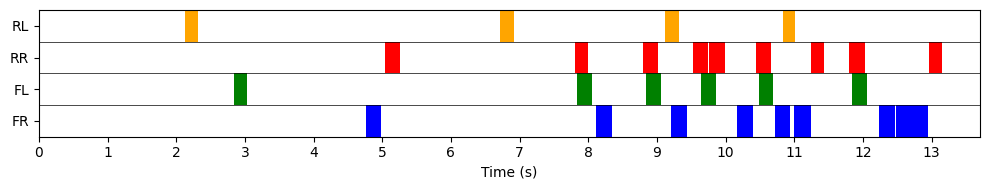
\includegraphics[width=0.85\textwidth]{images/data/swing-schedule.png}
  \caption{Example swing schedule from the preliminary simulation
    framework. Each row is one leg, and colored intervals indicate
    swing. Before \corlSwingScheduleTransitionMark\,s, the robot is
    commanded at low velocity and steps one foot at a time. After the
    command increases, swings overlap without a fixed alternating
    pattern.}
  \label{fig:data-swing-schedule}
\end{figure*}

\begin{figure}[t]
  \centering
  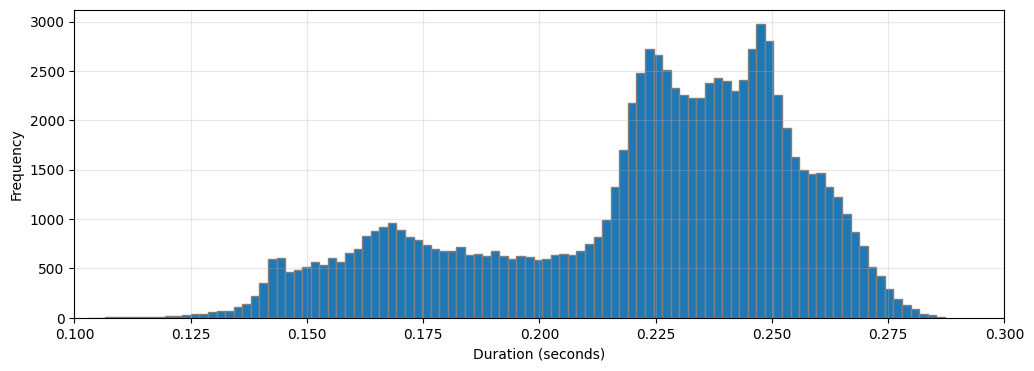
\includegraphics[width=\linewidth]{images/data/swing_duration_histogram.png}
  \caption{Swing durations selected by GaitNet during preliminary
    simulation evaluation.}
  \label{fig:data-swing-duration-histogram}
\end{figure}

\subsection{Simulation Results (Preliminary Framework)}
\label{subsec:results-simulation}

Before the hardware system in \autoref{sec:methodology}, previous
work \cite{Sullivan2025} evaluated cost-ablated
GaitNet in NVIDIA Isaac Lab. It compared GaitNet with an independent
single-leg baseline planner. The simulation grid covered terrain
difficulties from $\corlDifficultyMin\%$ to $\corlDifficultyMax\%$ in
$\corlDifficultyStep\%$ increments. It also covered commanded forward
velocities from $\corlVelocityMin$ to $\corlVelocityMax$\,m/s. Each
grid cell used \corlSimTrialsPerCell{} trials of
\corlSimEpisodeDuration\,s.

Those experiments used the sampled candidate distribution described in
\autoref{subsec:methodology-gaitnet-training}. Each decision compared
\corlTrainCandidatesPerLeg{} sampled candidates per leg and one
no-action option. They did not use the exhaustive
deployment-time enumeration introduced in
\autoref{subsec:methodology-gaitnet-selection}. We therefore report
the simulation results as evidence for the original mechanism. They
are not a direct validation of the deployed enumeration procedure.

In that preliminary setting, GaitNet (Full) reached a
$\corlResCostAblatedSurvivalRate\%$ mean survival rate. The
independent single-leg baseline reached
$\corlResBaselineSurvivalRate\%$. The baseline selected the lowest-cost
foothold. It moved one leg at a time and used a fixed
$\corlBaselineSwingDurationMs$\,ms swing duration. Its structure is
closest to the GaitNet-Single hardware ablation, but it has no learned
value function. GaitNet stayed strong below
$\corlStrongPerfVelocityThreshold$\,m/s. The baseline degraded as
commanded velocity and terrain difficulty increased. The gap was
smallest on flat ground at the lowest speed, where concurrent
high-rate footstep selection matters least.

\subsection{Emergent Concurrency Analysis (Preliminary Framework)}
\label{subsec:results-concurrency}

The preliminary simulations also show the mechanism behind the
hardware ablations. \autoref{fig:data-swing-schedule} shows one
representative swing schedule. At low commanded velocity, before
\corlSwingScheduleTransitionMark\,s, GaitNet moves one foot at a time.
When the command speed increases, it starts new swings before earlier
swings finish. The overlap does not follow a fixed alternating
pattern.

No mode switch or gait change triggers this transition. The same value
function and no-action comparison govern both regimes. Higher
commanded velocity simply makes useful footholds beat the no-action
score more often while another leg is already in the air.
Deployment-time enumeration changes which candidates are
available for comparison. It does not change how any individual
candidate is ranked. We therefore expect the same decision mechanism
to remain under dense enumeration. The hardware comparison tests that
expectation directly.

\autoref{fig:data-swing-duration-histogram} shows that the duration
head remains active. During typical forward motion, selected swing
durations peak between $\corlSwingHistPeakMin$\,s and
$\corlSwingHistPeakMax$\,s. There is also a secondary mode near
$\corlSwingHistSecondaryMode$\,s for faster situational steps, such as
recovery from marginal footholds. Across training, the mean selected
duration is $\corlResMeanSwingDuration$\,s with standard deviation
$\corlResStdSwingDuration$\,s. This shows that the duration output
does not collapse to a constant.

\subsection{Swing Duration Ablation (Preliminary Framework)}
\label{subsec:results-duration-ablation}

The preliminary framework \cite{Sullivan2025} also tested whether
learned swing duration was needed under the evaluated conditions. The
duration-ablated model was trained like standard GaitNet. The only
difference was that its swing duration was fixed to
$\corlResDurationAblationFixedDuration$\,s. This is close to the mean
duration selected by the learned model.

The ablation produced a null result. Duration-Ablated-GaitNet reached
a $\corlResDurationAblatedSurvivalRate\%$ survival rate. This was
statistically indistinguishable from the
$\corlResGaitNetSurvivalRate\%$ survival rate of the matched standard
model. We do not take this to mean that swing-duration selection is
always unimportant. More likely, the tested terrain and velocity
ranges did not require the full duration range. The reward also did
not explicitly encourage timing variation beyond what was needed to
avoid termination. The duration head is inexpensive, and it may matter
at higher speeds or on harder terrain. We therefore keep it in the
architecture evaluated in this paper.
